\documentclass[11pt,a4paper]{article}

\usepackage[T1]{fontenc}
\usepackage[utf8]{inputenc}
\usepackage[french]{babel}
\usepackage{lmodern}
\usepackage{geometry}
\usepackage{setspace}
\usepackage{amsmath, amssymb, amsfonts}
\usepackage{booktabs}
\usepackage{longtable}
\usepackage{array}
\usepackage{graphicx}
\usepackage{float}
\usepackage{caption}
\usepackage{subcaption}
\usepackage{hyperref}
\usepackage{xcolor}
\usepackage{enumitem}

\geometry{margin=2.5cm}
\setstretch{1.15}
\hypersetup{colorlinks=true,linkcolor=blue,citecolor=blue,urlcolor=blue}

\title{Comparaison de la qualite de modelisation de l'incertitude\\
\large Auto-encodeur vs modele de classification}
\author{Projet de recherche de fin d'etudes -- MOSAIK\\
LORIA, equipe MosAIk}
\date{20 mars 2026}

\begin{document}

\maketitle
\tableofcontents
\newpage

\section{Resume}
Ce rapport presente une etude complete de la qualite de modelisation de l'incertitude entre des modeles supervises de classification et des auto-encodeurs. L'hypothese centrale est qu'une contrainte forte de prediction d'etiquette peut detruire une partie de l'information utile a la quantification d'incertitude epistemique. Le travail est structure en trois volets: (i) demonstration experimentale sur donnees reelles (MNIST, Fashion-MNIST, Cat-Dog-Bird), (ii) preuve empirique par simulation controlee sur donnees synthetiques, (iii) ouverture vers une preuve formelle.

Les principaux constats sont les suivants:
\begin{itemize}[leftmargin=1.2cm]
    \item Sur MNIST, les modeles supervises atteignent de hautes performances de classification, en particulier le CNN (accuracy 99.14\%).
    \item Sur Cat-Dog, le CNN surpasse nettement le MLP (accuracy 82.23\% vs 69.03\%), ce qui influence la qualite des representations 32D utilisees ensuite pour la detection OOD via Random Forest.
    \item La campagne de simulation extreme ratio sweep confirme une relation croissante entre ratio de compression et qualite de preservation d'information (Spearman), avec une tendance quasi lineaire en echelle semi-logarithmique.
\end{itemize}

\section{Introduction et contexte scientifique}
\subsection{Problematique}
Le cadre de depart du projet est: comparer la qualite de modelisation de l'incertitude d'un auto-encodeur versus un classifieur multi-classes. L'intuition est que le classifieur est force d'optimiser une variable cible discrete (classe), ce qui peut comprimer les representations internes d'une maniere qui preserve bien la decision, mais moins bien la structure probabiliste globale de l'entree.

\subsection{Hypothese de recherche}
L'hypothese testee est une \textbf{perte d'information sur l'incertitude epistemique} lorsque l'on impose la prediction d'etiquettes. L'auto-encodeur, optimise pour reconstruire les donnees, est suppose conserver davantage d'information utile a la caracterisation du voisinage et des zones de faible support des donnees.

\subsection{Positionnement dans la litterature}
Le projet s'inscrit dans les approches de quantification d'incertitude relevant notamment:
\begin{itemize}[leftmargin=1.2cm]
    \item des methodes bayesiennes,
    \item des methodes ensemblistes,
    \item des methodes evidentielles / risque d'ordre superieur,
    \item des methodes fondees sur la densite locale.
\end{itemize}
La contribution pratique ici est de relier ces idees a un pipeline experimental coherent et reproductible, avec comparaison directe de representations latentes.

\section{Organisation du travail et artefacts du depot}
Le depot comporte:
\begin{itemize}[leftmargin=1.2cm]
    \item \textbf{demonstration}: notebook principal de comparaison sur jeux reels, plus briques de modeles et methodes d'incertitude.
    \item \textbf{preuve\_empirique}: simulation massive controlee via \textit{extreme ratio sweep} et execution SLURM.
    \item \textbf{preuve\_formelle}: socle de documentation theorique.
    \item \textbf{comptes\_rendus}: trace des choix de cadrage scientifique et des decisions de projet.
\end{itemize}

\section{Volet 1 -- Demonstration sur donnees reelles}
\subsection{Notebook central}
Le notebook \textit{demo\_quant\_incertitudes.ipynb} est organise en 51 cellules (28 code, 23 markdown) en deux blocs experimentaux:
\begin{enumerate}[leftmargin=1.2cm]
    \item bloc MNIST/Fashion-MNIST,
    \item bloc Cat-Dog-Bird.
\end{enumerate}

\subsection{Bloc MNIST/Fashion-MNIST}
\subsubsection{Donnees et pretraitement}
Le chargement utilise \texttt{torchvision.datasets.MNIST} et \texttt{FashionMNIST}, avec transformation:
\begin{equation}
\text{Normalize}(x;\mu=0.1307,\sigma=0.3081).
\end{equation}
Batch size: 128.

\subsubsection{Modeles entraines}
Quatre modeles sont entrainees sur MNIST:
\begin{itemize}[leftmargin=1.2cm]
    \item \textbf{MLP supervise} (4 epochs):
    \begin{equation}
    784 \rightarrow 512 \rightarrow 256 \rightarrow 128 \rightarrow 64 \rightarrow 32 \rightarrow 10.
    \end{equation}
    \item \textbf{CNN supervise} (5 epochs):
    \begin{equation}
    \text{Conv}(1,32) \rightarrow \text{Conv}(32,64) \rightarrow \text{MaxPool} \rightarrow \text{Conv}(64,128) \rightarrow \text{MaxPool} \rightarrow \text{FC}(128\cdot7\cdot7\rightarrow256\rightarrow128\rightarrow32\rightarrow10).
    \end{equation}
    \item \textbf{Auto-encodeur MLP} (10 epochs): encodeur 784\(\to\)512\(\to\)256\(\to\)128\(\to\)64\(\to\)32, decodeur symetrique vers 784.
    \item \textbf{Auto-encodeur CNN} (10 epochs): encodeur convolutionnel, bottleneck lineaire 32D, decodeur en convolutions transposees vers image 28\(\times\)28.
\end{itemize}

Optimisation: Adam (lr = 1e-3). Pertes: CrossEntropy pour modeles supervises, MSE pour auto-encodeurs.

\subsubsection{Comparaison supervisee MLP vs CNN}
A partir des matrices de confusion observees dans le notebook, les metriques derivees sont:
\begin{itemize}[leftmargin=1.2cm]
    \item \textbf{MLP MNIST}: accuracy 97.64\%, precision macro 97.65\%, recall macro 97.60\%, F1 macro 97.62\%.
    \item \textbf{CNN MNIST}: accuracy 99.14\%, precision macro 99.14\%, recall macro 99.13\%, F1 macro 99.13\%.
\end{itemize}
Le gain du CNN est coherent avec sa meilleure adequation aux structures spatiales des images.

\subsubsection{Pipeline d'incertitude via representations 32D}
Pour chaque famille de modele, une representation 32D est extraite:
\begin{itemize}[leftmargin=1.2cm]
    \item MLP: sortie de \textit{net[:-1]}.
    \item CNN: sortie de \textit{classifier[:-1](features(x))}.
    \item AE-MLP: sortie encodeur.
    \item AE-CNN: sortie bottleneck.
\end{itemize}

Ces representations sont sauvegardees pour:
\begin{itemize}[leftmargin=1.2cm]
    \item MNIST train/test,
    \item Fashion-MNIST test (utilise comme OOD).
\end{itemize}

Un Random Forest (200 arbres, \texttt{min\_samples\_leaf}=5) est entraine sur MNIST train 32D, puis evalue sur MNIST test (ID) et Fashion test (OOD). Deux quantifications epistemiques sont codees:
\begin{enumerate}[leftmargin=1.2cm]
    \item variance inter-arbres des probabilites predictives,
    \item information mutuelle (entropie de la moyenne moins moyenne des entropies).
\end{enumerate}

\paragraph{Interpretation scientifique}
Le protocole est pertinent pour tester l'hypothese: si une representation preserve mieux la structure de densite des donnees, elle doit faciliter la separation des distributions d'incertitude ID/OOD. Les histogrammes de densite produits dans le notebook montrent justement cette separation comparee sur les 4 representations.

\subsection{Bloc Cat-Dog-Bird}
\subsubsection{Donnees et pretraitement}
Le notebook telecharge un dataset Kaggle \textit{high-resolution-catdogbird-image-dataset-13000} et detecte automatiquement la racine ImageFolder contenant \textit{cat}, \textit{dog}, \textit{bird}.

Transformation:
\begin{equation}
\text{Resize}(64,64),\quad \text{Normalize}(\mu=[0.485,0.456,0.406],\sigma=[0.229,0.224,0.225]).
\end{equation}

Comptages observes:
\begin{itemize}[leftmargin=1.2cm]
    \item Cats: 4015,
    \item Dogs: 5180,
    \item Birds: 4149 (OOD).
\end{itemize}

Entrainement supervise sur Cats+Dogs uniquement (binaire), puis evaluation OOD sur Birds.

\subsubsection{Modeles}
Quatre modeles analogues au bloc MNIST:
\begin{itemize}[leftmargin=1.2cm]
    \item MLP CDB (4 epochs): entree 64\(\times\)64\(\times\)3, sorties binaires.
    \item CNN CDB (5 epochs): conv 3\(\to\)32\(\to\)64\(\to\)128, tete fully-connected vers 2 classes.
    \item AE-MLP CDB (10 epochs), bottleneck 32D.
    \item AE-CNN CDB (10 epochs), bottleneck 32D.
\end{itemize}

\subsubsection{Comparaison de performance Cat-Dog}
A partir des matrices de confusion du notebook:
\begin{itemize}[leftmargin=1.2cm]
    \item \textbf{MLP}: accuracy 69.03\%, precision macro 68.58\%, recall macro 67.79\%, F1 macro 67.95\%.
    \item \textbf{CNN}: accuracy 82.23\%, precision macro 82.92\%, recall macro 81.02\%, F1 macro 81.50\%.
\end{itemize}

Le CNN apprend des motifs visuels plus robustes, ce qui est attendu sur image couleur 64\(\times\)64.

\subsubsection{Quantification d'incertitude sur CDB}
Le meme schema que MNIST est applique:
\begin{enumerate}[leftmargin=1.2cm]
    \item extraction de representations 32D,
    \item apprentissage RF sur Cat+Dog,
    \item comparaison incertitude sur ID (Cat+Dog) versus OOD (Bird).
\end{enumerate}
Deux estimateurs epistemiques sont traces (variance inter-arbres et information mutuelle basee sur entropie).

\paragraph{Interpretation}
La detection OOD dans un regime inter-classes semantiquement proches (animaux domestiques vs oiseaux) est plus difficile que MNIST/Fashion-MNIST. L'interet du protocole est de tester la robustesse des representations dans un contexte moins "propre" qu'un benchmark de chiffres.

\section{Volet 2 -- Preuve empirique par simulation controlee}
\subsection{Objectif de la simulation}
Le script \textit{extreme\_ratio\_sweep\_v1.py} cherche a mesurer, sur donnees synthetiques controlees, l'effet du ratio de compression:
\begin{equation}
\rho = \frac{\text{dimension bottleneck}}{\text{dimension entree}}.
\end{equation}

L'indicateur principal est la correlation de Spearman entre:
\begin{itemize}[leftmargin=1.2cm]
    \item la log-densite vraie des donnees, $\log p_X(x)$,
    \item une densite estimee dans l'espace latent, $\log p_Z(z)$ (KDE gaussien).
\end{itemize}

\subsection{Construction des donnees}
Chaque repetition genere un melange de gaussiennes multivariees:
\begin{itemize}[leftmargin=1.2cm]
    \item 2 blobs,
    \item covariance vraie de rang faible (rang = 2) avec bruit diagonal,
    \item 10 000 echantillons,
    \item dimensions candidates de 16 a 200.
\end{itemize}

\subsection{Modele probabiliste entrainable}
Le modele est un auto-encodeur probabiliste:
\begin{itemize}[leftmargin=1.2cm]
    \item encodeur MLP: entree $d \to 48 \to 48 \to z$,
    \item decodeur produisant une moyenne $\mu(x)$ et une covariance
    \begin{equation}
    \Sigma = VV^\top + \mathrm{diag}(d),
    \end{equation}
    decomposee rang-faible + diagonale.
\end{itemize}

Perte optimisee: negative log-vraisemblance gaussienne multivariee.

\subsection{Plan d'experience}
\begin{itemize}[leftmargin=1.2cm]
    \item 30 ratios tests,
    \item 50 repetitions cibles,
    \item 60 epochs max par entrainement,
    \item early stopping (patience 8, delta 1e-3),
    \item batch size 256, Adam lr 1e-3, weight decay 1e-5.
\end{itemize}

Pour chaque repetition et ratio, on calcule Spearman puis on agrège les statistiques par ratio.

\subsection{Execution HPC et journalisation}
La soumission est automatisee via \textit{submit-slurm.py} et \textit{job.sbatch}:
\begin{itemize}[leftmargin=1.2cm]
    \item partition \textit{gpu\_prod\_long},
    \item limite de temps 12h,
    \item logs SLURM diriges vers \textit{logslurms/slurm-<job>\_<task>.out/.err},
    \item synchronisation des sorties vers \textit{extreme\_ratio\_sweep\_v1\_outputs/run\_<job>\_<task>}.
\end{itemize}

\subsection{Resultats observables sur la run partielle}
La run 159664\_1 s'est arretee par \textit{TIMEOUT} apres 12h. Un CSV partiel a ete sauvegarde puis rejoue localement.

Donnees effectivement exploitees:
\begin{itemize}[leftmargin=1.2cm]
    \item 1440 observations,
    \item 48 repetitions completes,
    \item 30 ratios uniques,
    \item ratios de 0.01 a 1.0.
\end{itemize}

Statistiques globales (replay):
\begin{itemize}[leftmargin=1.2cm]
    \item Spearman global moyen: 0.2489,
    \item Spearman global ecart-type: 0.1349,
    \item meilleur ratio moyen: 0.8333 (Spearman moyen 0.4644),
    \item plus faible ratio moyen: 0.01 (Spearman moyen 0.0423).
\end{itemize}

Linearity semi-log:
\begin{itemize}[leftmargin=1.2cm]
    \item pente de la courbe moyenne: 0.2504,
    \item intercept: 0.3732,
    \item $R^2$ de la courbe moyenne: 0.7495,
    \item $R^2$ moyen repetition-par-repetition: 0.7145 $\pm$ 0.0211,
    \item quantiles $R^2$: Q10 = 0.6927, mediane = 0.7137, Q90 = 0.7315.
\end{itemize}

\paragraph{Interpretation}
Ces valeurs indiquent une relation positive robuste entre ratio de compression et preservation de la structure de densite dans le latent. L'echelle semi-log rend visible une croissance proche d'un modele affine en $\log_{10}(\rho)$, compatible avec l'idee d'une degradation non lineaire lorsque la compression devient extreme.

\begin{figure}[H]
    \centering
    \IfFileExists{../preuve_empirique/extreme_ratio_sweep_v1_outputs/run_159664_1/extreme_ratio_sweep_replayed.png}{%
        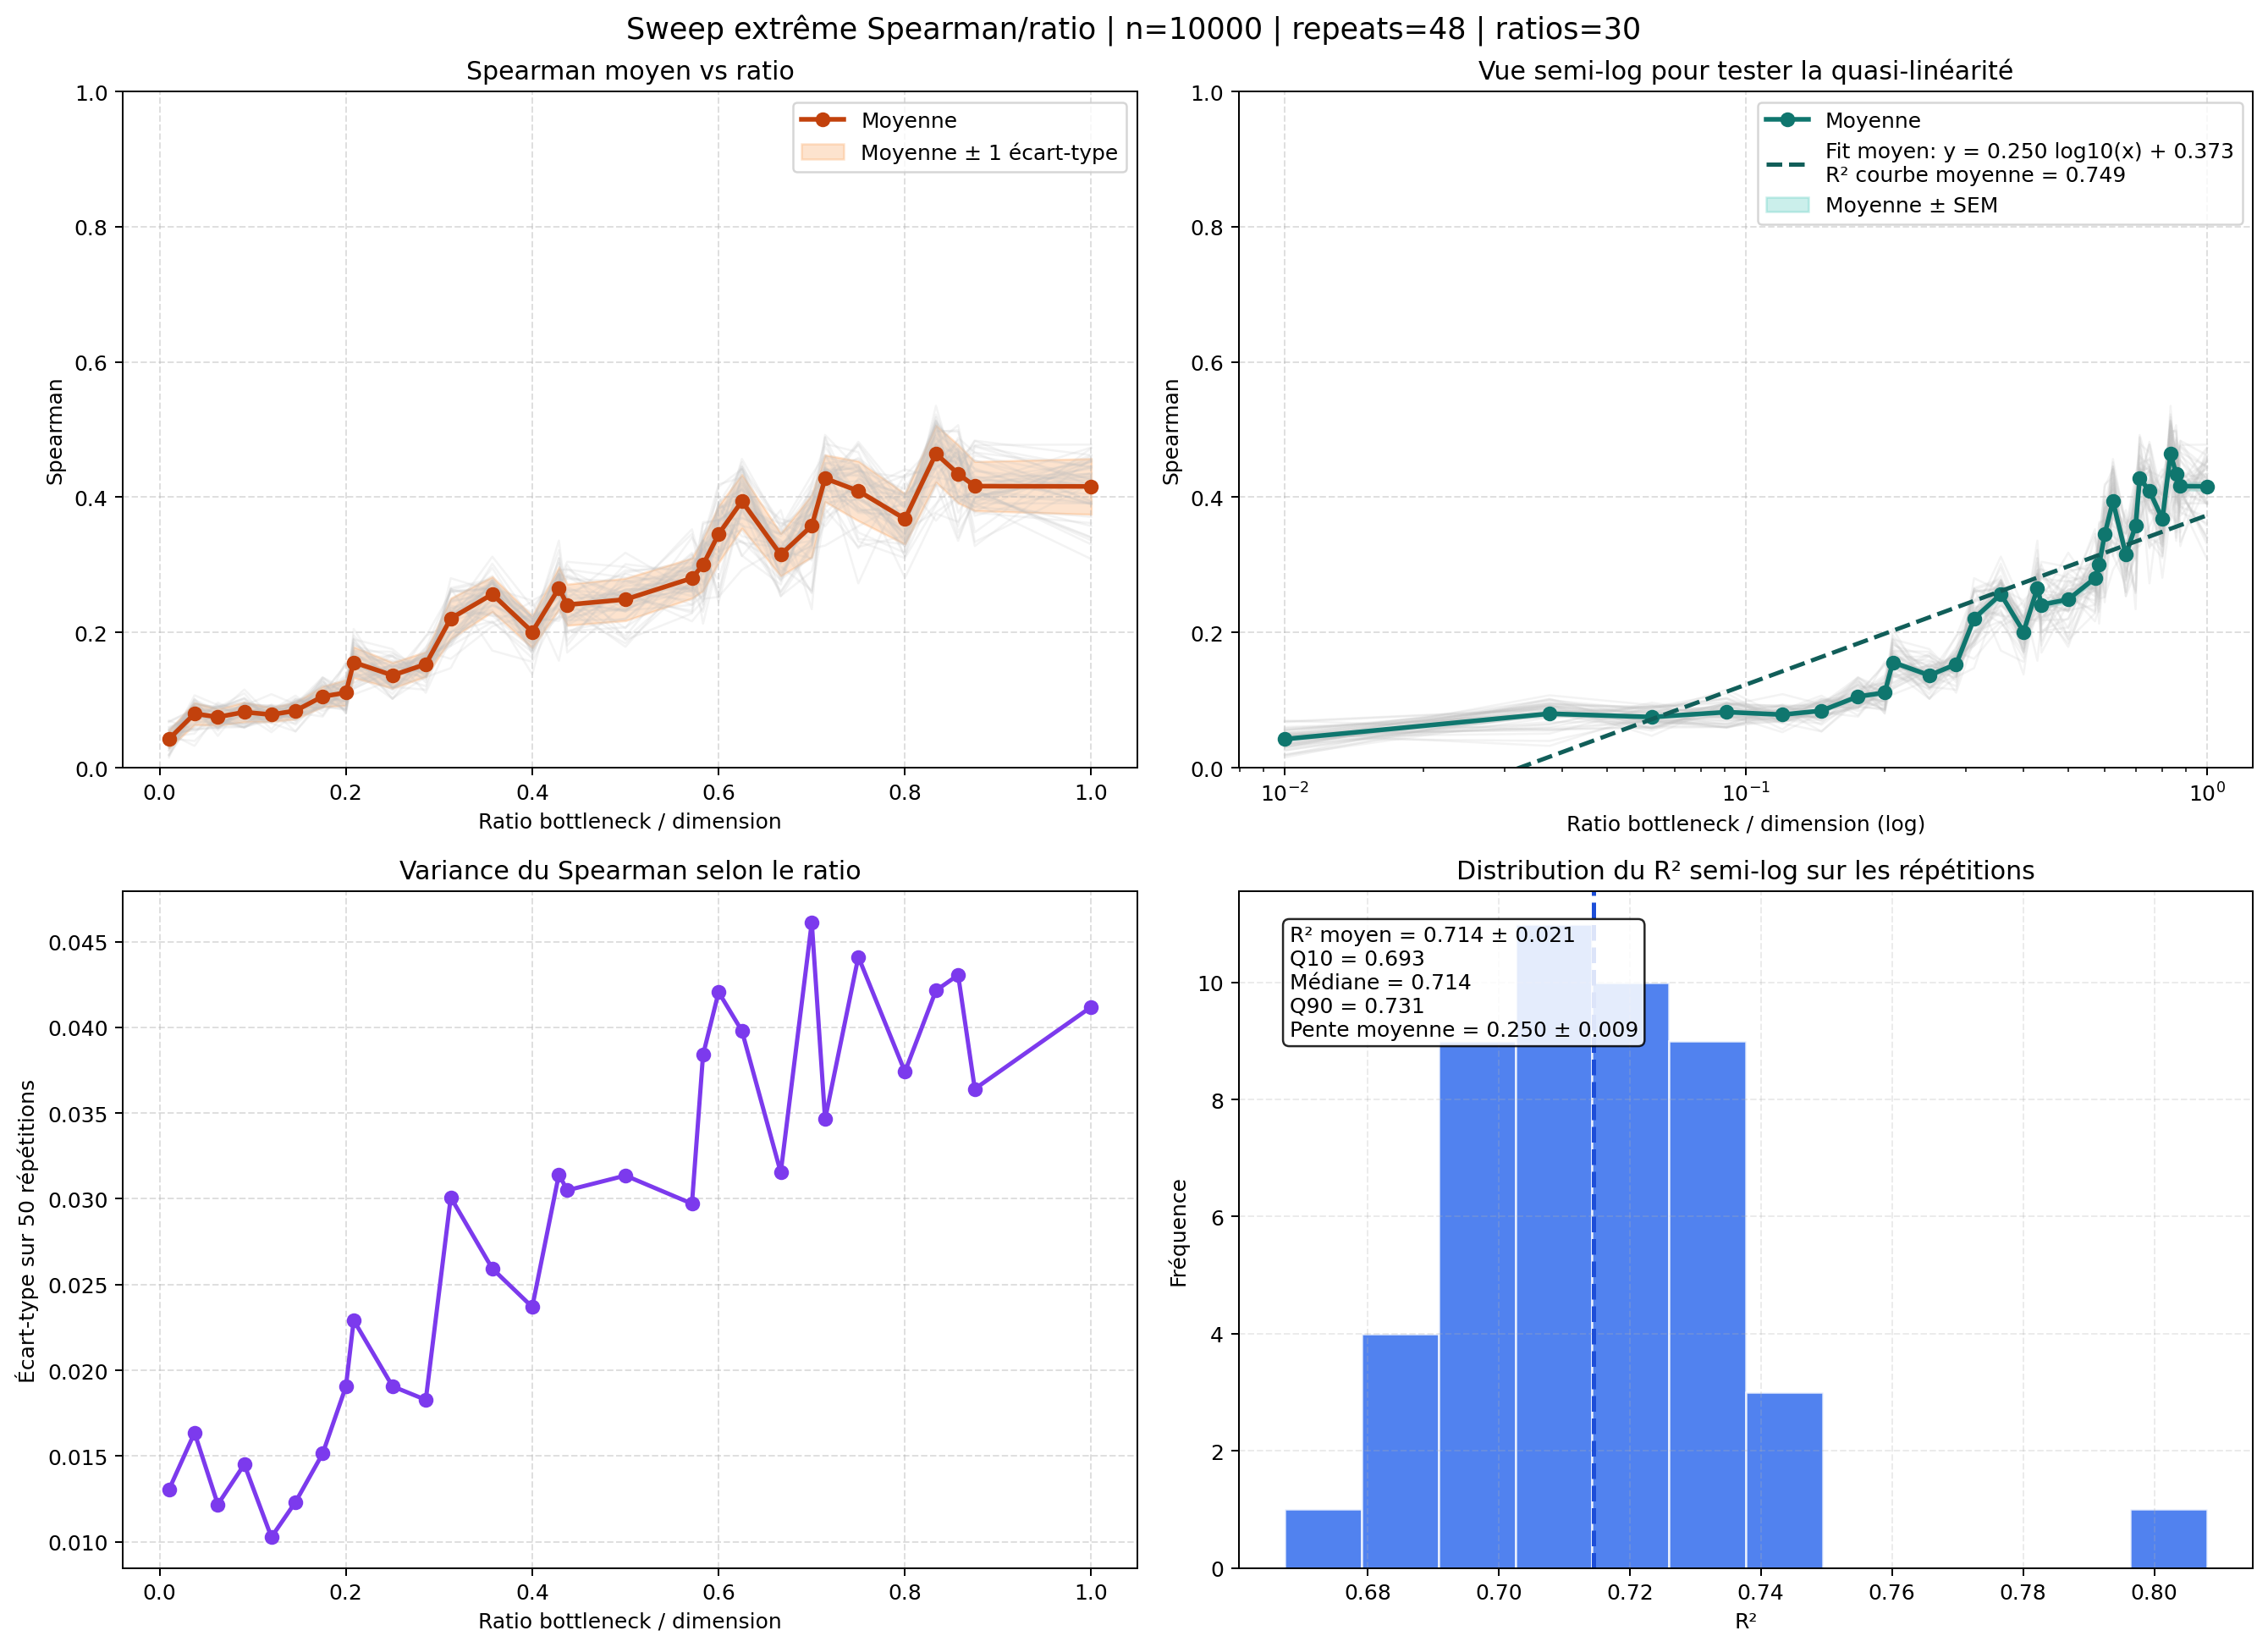
\includegraphics[width=0.95\textwidth]{../preuve_empirique/extreme_ratio_sweep_v1_outputs/run_159664_1/extreme_ratio_sweep_replayed.png}
        \caption{Reconstruction des sorties du extreme ratio sweep a partir du fichier partiel.}
    }{%
        \fbox{\parbox{0.9\textwidth}{Figure non trouvee localement. Le rapport reste compilable sans cette illustration.}}
        \caption{Placeholder figure extreme ratio sweep.}
    }
\end{figure}

\section{Volet 3 -- Element de preuve formelle}
Le dossier preuve formelle contient principalement le cadrage documentaire de la demonstration mathematique attendue. Le plan conceptuel est bien pose:
\begin{itemize}[leftmargin=1.2cm]
    \item formaliser la decomposition des incertitudes,
    \item caracteriser la contrainte de classification comme projection d'information,
    \item montrer la perte potentielle d'information sur la structure de densite.
\end{itemize}

Ce volet est a completer par les derivations explicites (theoremes, hypotheses, preuves), mais la direction scientifique est coherente avec les evidences empiriques deja obtenues.

\section{Discussion scientifique}
\subsection{Ce que les resultats supportent clairement}
\begin{enumerate}[leftmargin=1.2cm]
    \item Les representations latentes dependent fortement de l'objectif d'apprentissage (classification vs reconstruction).
    \item La qualite de classification pure n'est pas un proxy suffisant de qualite de modelisation de l'incertitude.
    \item Le test de stress sur ratio de compression montre une dynamique reguliere et quantifiable de la perte de structure informationnelle.
\end{enumerate}

\subsection{Ce qui reste ouvert}
\begin{enumerate}[leftmargin=1.2cm]
    \item Generalisation a d'autres donnees (medical, vision haute resolution, series temporelles).
    \item Comparaison avec alternatives bayesiennes explicites (Laplace, MC Dropout, Deep Ensembles) sur un protocole identique end-to-end.
    \item Finalisation d'une preuve theorique complete pour relier observations numeriques et bornes informationnelles.
\end{enumerate}

\subsection{Limites}
\begin{itemize}[leftmargin=1.2cm]
    \item Une run HPC interrompue (48/50 repetitions) sur le sweep extreme.
    \item Certaines metriques de notebook ne sont pas exportees automatiquement en CSV; une partie des chiffres est issue des matrices de confusion persistees.
    \item Pas de benchmark multi-seeds systematique sur l'ensemble des experiences notebook.
\end{itemize}

\section{Recommandations pour version conference}
\begin{enumerate}[leftmargin=1.2cm]
    \item Rejouer la simulation complete (50/50) et ajouter intervalles de confiance bootstrap par ratio.
    \item Standardiser un protocole OOD commun pour tous modeles et toutes representations (AUROC, AUPR, FPR95).
    \item Ajouter une section ablation: largeur du latent, type de decodeur, bandwidth KDE, nombre d'arbres RF.
    \item Integrer un volet statistique inferentiel (tests de differences de moyennes corrigees multiplicite).
    \item Transformer le notebook en pipeline scriptable reproduisible (Hydra/CLI + logs versionnes).
\end{enumerate}

\section{Conclusion}
Le projet valide deja une base experimentale solide pour soutenir l'hypothese de perte d'information sous contrainte de classification. Les experiences sur donnees reelles montrent des comportements differencies entre modeles supervises et auto-encodeurs. La simulation controlee renforce ce constat en quantifiant explicitement l'effet de la compression sur la preservation de la structure de densite.

L'ensemble constitue une fondation credible pour une soumission de type workshop/short paper, a condition de finaliser: (i) la campagne complete, (ii) les metriques OOD harmonisees, (iii) la formalisation theorique.

\appendix
\section{Annexe A -- Hyperparametres principaux}
\begin{longtable}{p{4.2cm}p{10.5cm}}
\toprule
Bloc & Valeurs \\
\midrule
MNIST MLP & Adam, lr=1e-3, 4 epochs, architecture 784-512-256-128-64-32-10 \\
MNIST CNN & Adam, lr=1e-3, 5 epochs, Conv(1,32)-Conv(32,64)-Pool-Conv(64,128)-Pool-FC-10 \\
MNIST AE-MLP & Adam, lr=1e-3, 10 epochs, bottleneck 32 \\
MNIST AE-CNN & Adam, lr=1e-3, 10 epochs, bottleneck lineaire 32 \\
CDB MLP/CNN & Entrée 64x64x3, classification binaire Cat vs Dog, epochs 4/5 \\
CDB AE & Versions MLP et CNN, bottleneck 32, epochs 10 \\
RF UQ & 200 arbres, min\_samples\_leaf=5, evaluation ID vs OOD \\
Extreme ratio sweep & 30 ratios, 50 repetitions cibles, 10 000 echantillons, hidden=48, epochs=60, patience=8 \\
\bottomrule
\end{longtable}

\section{Annexe B -- Commandes utiles de reproduction}
\begin{itemize}[leftmargin=1.2cm]
    \item Execution locale du replay partiel: \texttt{python3 replay\_extreme\_ratio\_from\_partial.py --no-show}
    \item Soumission SLURM: \texttt{python3 submit-slurm.py --nruns 1}
    \item Notebook principal: \texttt{jupyter notebook demonstration/demo\_quant\_incertitudes.ipynb}
\end{itemize}

\section{Annexe C -- Espace reserve}
Annexe volontairement laissee vide pour ajout futur: preuves detaillees, tableaux complements, resultats multi-seeds.

\section*{Abstract (francais)}
Ce travail etudie la qualite de modelisation de l'incertitude en comparant deux paradigmes d'apprentissage: la classification supervisee et la reconstruction non supervisee par auto-encodeur. L'hypothese centrale est qu'une contrainte forte de prediction d'etiquette peut induire une perte d'information utile a la quantification de l'incertitude epistemique. Pour l'evaluer, nous combinons des experiences sur donnees reelles (MNIST, Fashion-MNIST, Cat-Dog-Bird) et une campagne de simulation controlee a grande echelle fondee sur un balayage du ratio de compression latent. Sur les jeux reels, les modeles supervises obtiennent de tres bonnes performances de classification, mais la qualite des representations pour la separation ID/OOD depend fortement de l'architecture et de la nature des features extraites. Sur la preuve empirique, les resultats montrent une relation monotone croissante entre ratio de compression et preservation de structure informationnelle, mesuree par la correlation de Spearman entre densite vraie et densite estimee dans l'espace latent. La vue semi-logarithmique revele une tendance quasi lineaire robuste sur les repetitions observees, ce qui soutient l'idee d'une degradation progressive de la modelisation d'incertitude lorsque la compression devient extreme. Dans l'ensemble, les observations consolident l'hypothese de perte d'information sous contrainte de classification et etablissent une base experimentale solide en vue d'une formalisation theorique complete et d'une valorisation academique.

\end{document}
